\section{Demonstration by examples}
\label{section:evaluation}

\begin{table*}[b]
	\centering
	\renewcommand{\arraystretch}{1.3}
	\begin{tabularx}{\textwidth}{|Y|Y|Y|Y|}
		\hline

		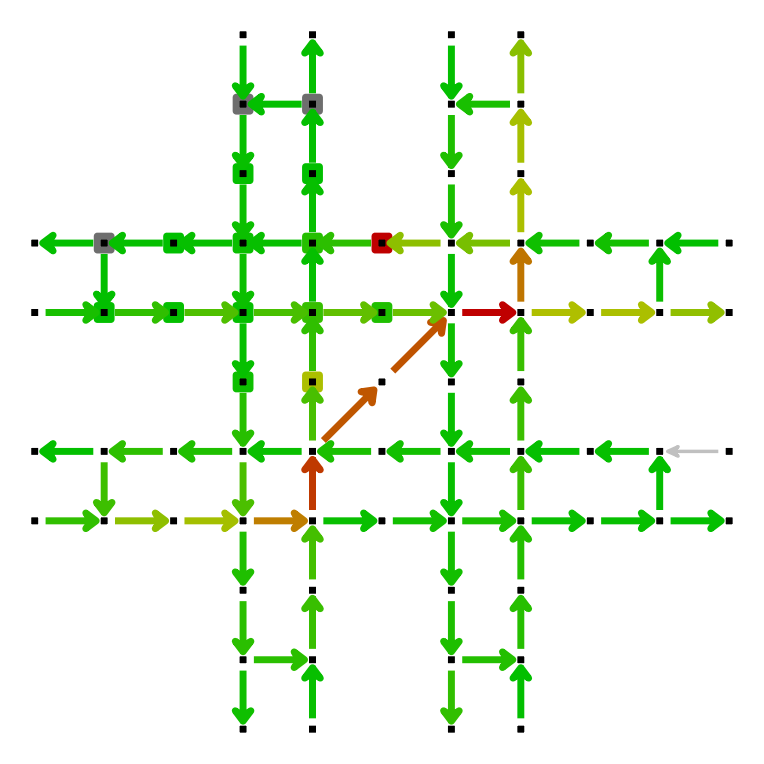
\includegraphics[trim=0 0 0 -4,scale=0.155]{../gfx/data/E1_003.png}  &
		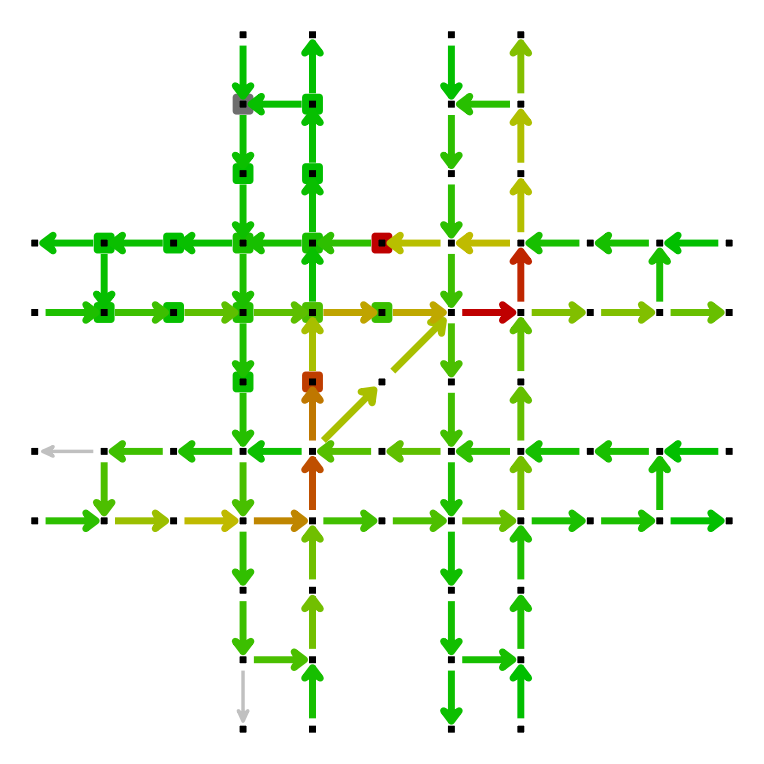
\includegraphics[trim=0 0 0 -4,scale=0.155]{../gfx/data/E2_003.png}  &
		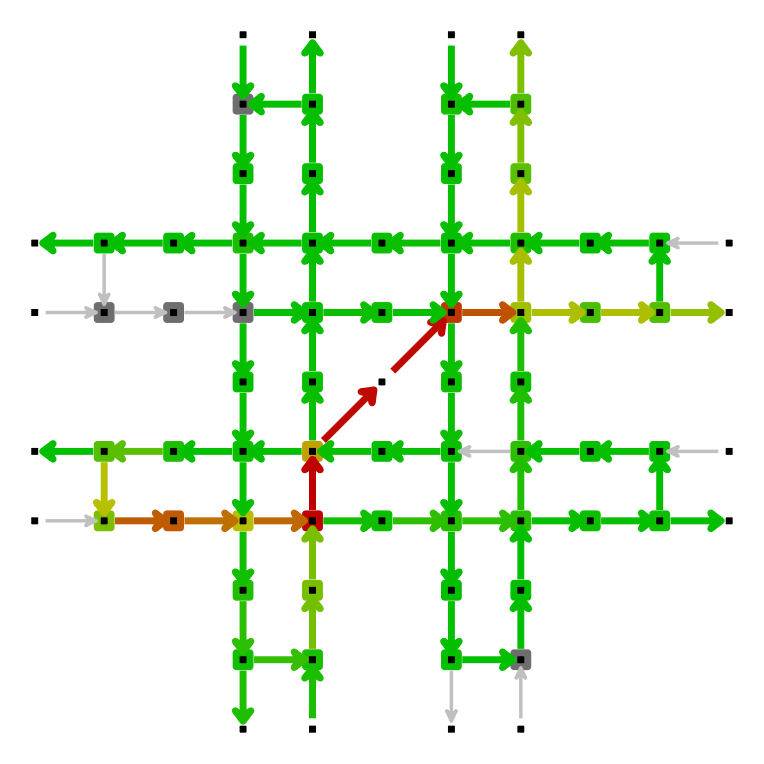
\includegraphics[trim=0 0 0 -4,scale=0.155]{../gfx/data/E3_003.png} &
		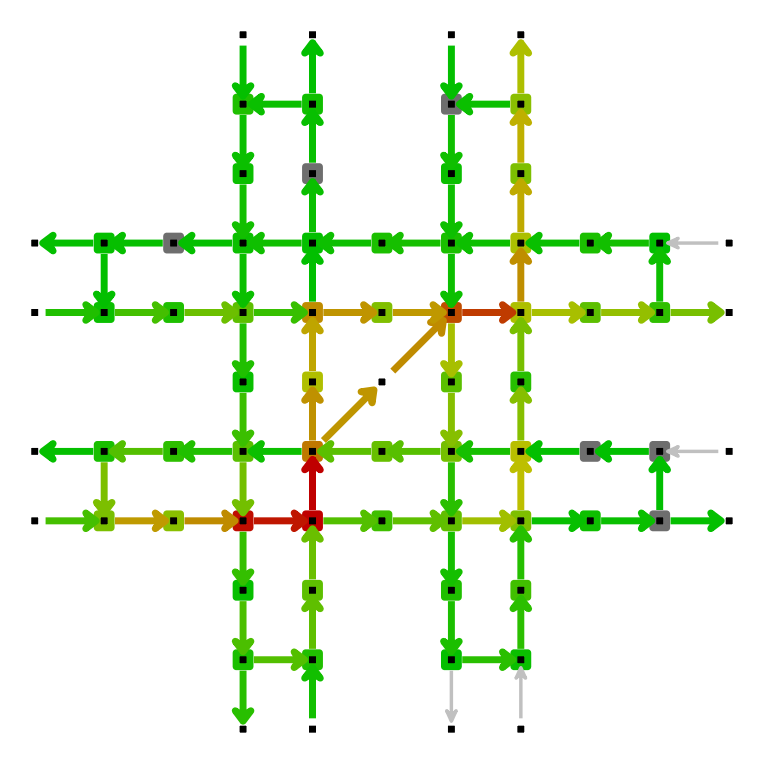
\includegraphics[trim=0 0 0 -4,scale=0.155]{../gfx/data/E4_003.png} \\ \hline
		
 		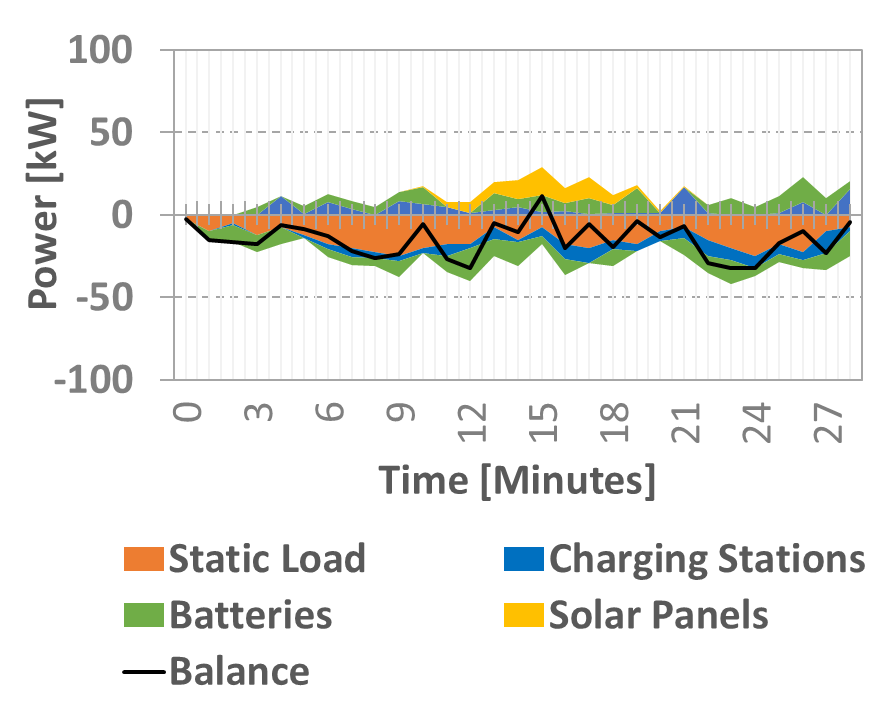
\includegraphics[trim=0 0 0 -3,scale=0.285]{../gfx/data/E1_001.png} &
		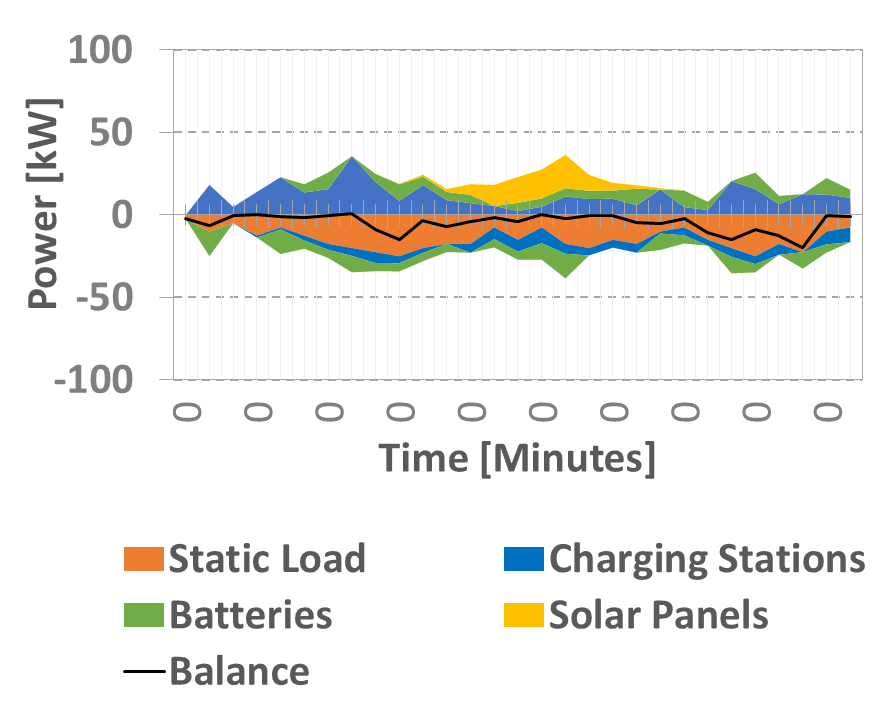
\includegraphics[trim=0 0 0 -3,scale=0.285]{../gfx/data/E2_001.png} &
		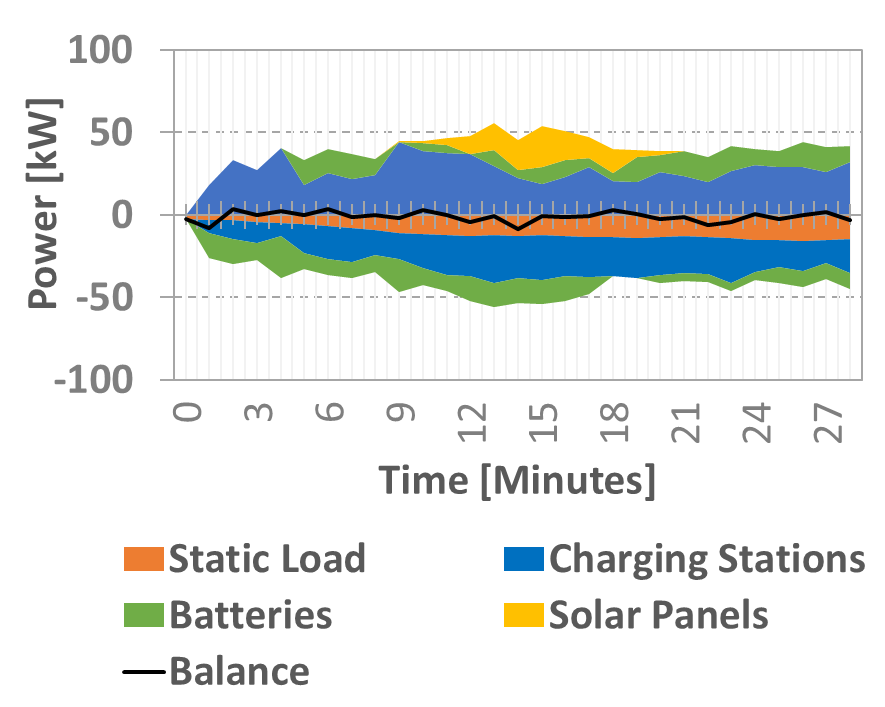
\includegraphics[trim=0 0 0 -3,scale=0.285]{../gfx/data/E3_001.png}  &
		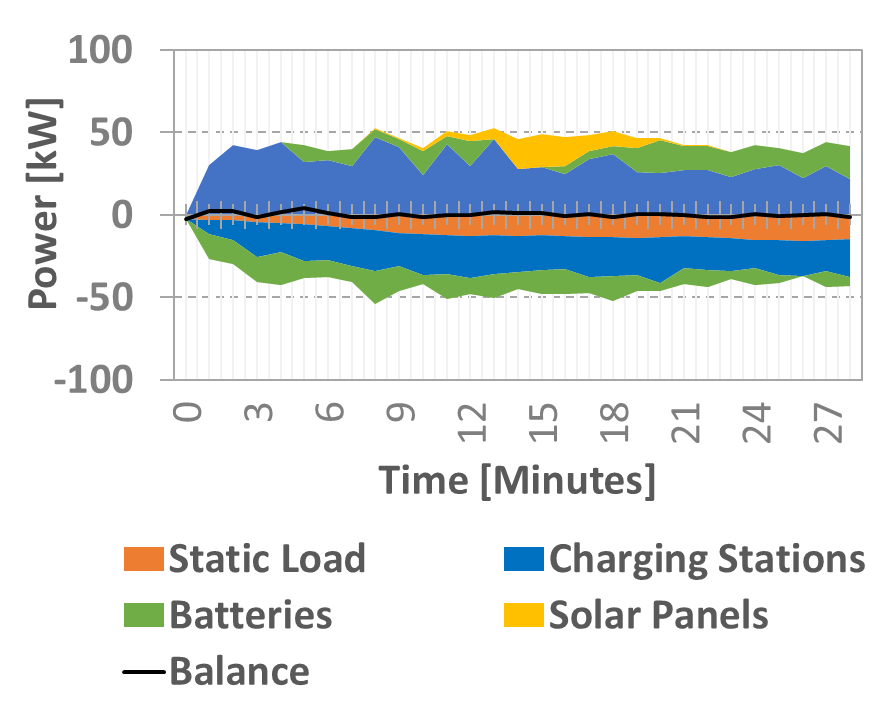
\includegraphics[trim=0 0 0 -3,scale=0.285]{../gfx/data/E4_001.png} \\ \hline
		
		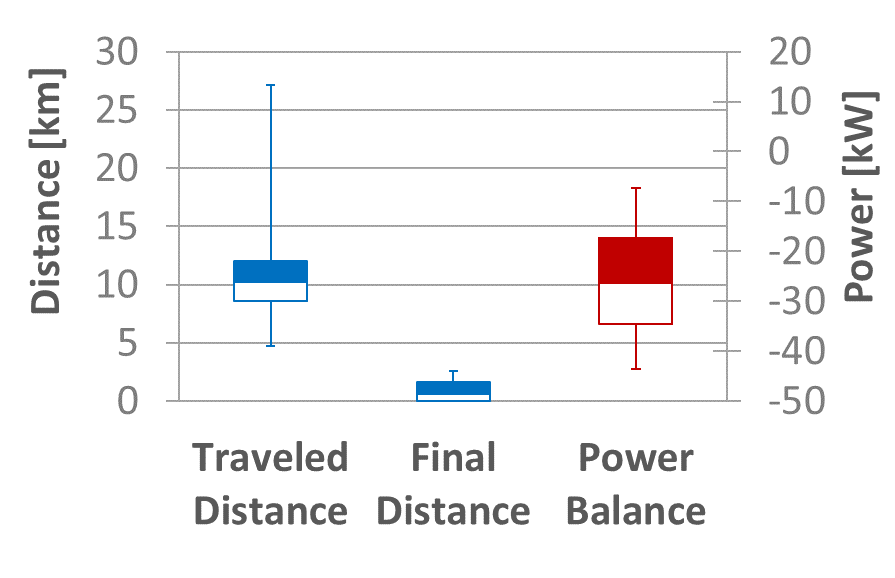
\includegraphics[trim=0 0 0 -3,scale=0.285]{../gfx/data/E1_002.png} &
		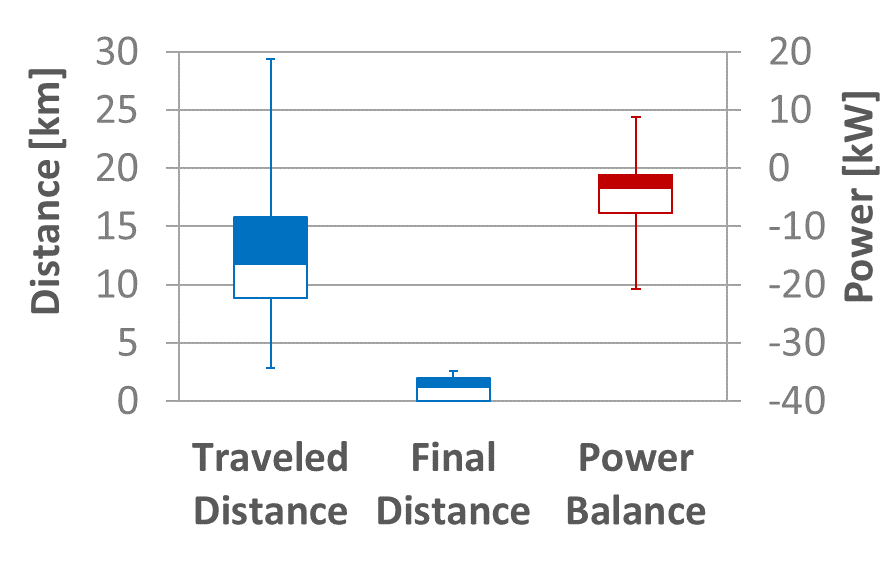
\includegraphics[trim=0 0 0 -3,scale=0.285]{../gfx/data/E2_002.png} &
		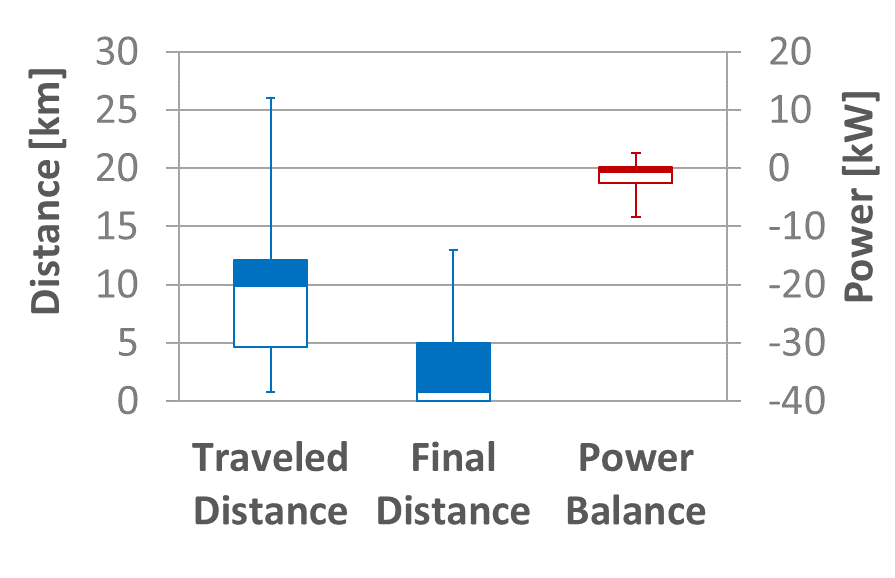
\includegraphics[trim=0 0 0 -3,scale=0.285]{../gfx/data/E3_002.png} &
		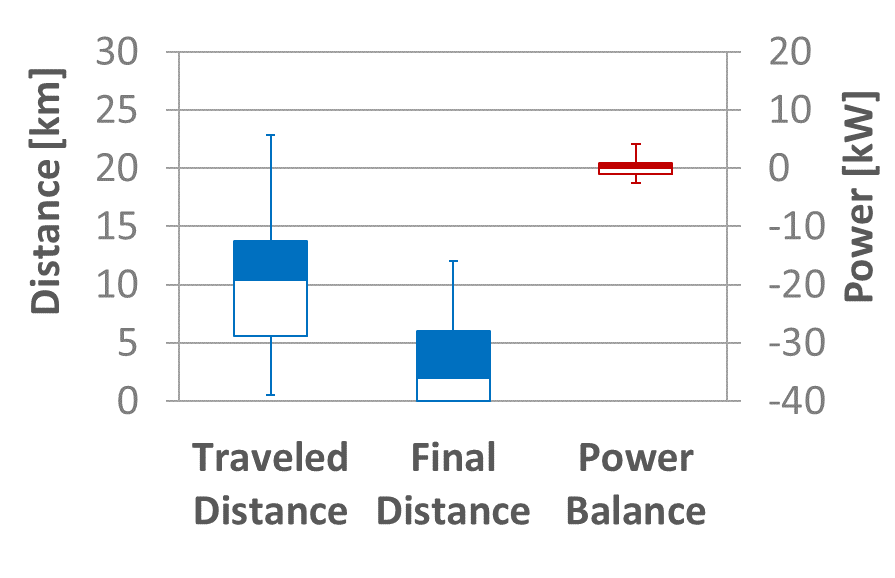
\includegraphics[trim=0 0 0 -3,scale=0.285]{../gfx/data/E4_002.png} \\ \hline
		
		\begin{tabulary}{4cm}{L|L}
		\textbf{Computation Time} & 229s \\
		\textbf{Memory Usage} & 6.03GB \\
		\textbf{Lines of Code (LOC)} & 350 \\
		\end{tabulary}
		&
		\begin{tabulary}{4cm}{L|L}
			\textbf{Computation Time} & 250s \\
			\textbf{Memory Usage} & 5.27GB \\
			\textbf{Lines of Code (LOC)} & 350 \\
		\end{tabulary}
		&
		\begin{tabulary}{4cm}{L|L}
			\textbf{Computation Time} & 218s \\
			\textbf{Memory Usage} & 6.41GB \\
			\textbf{Lines of Code (LOC)} & 350 \\
		\end{tabulary}
		&
		\begin{tabulary}{4cm}{L|L}
			\textbf{Computation Time} & 227s \\
			\textbf{Memory Usage} & 6.75GB \\
			\textbf{Lines of Code (LOC)} & 350 \\
		\end{tabulary}
		\\ \hline						
		
		\end{tabularx} 
	
	\caption{Estimated system behavior for all four scenarios illustrated by energy and cost charts and aggregated traffic graphs.}
	\label{figure:examples}
\end{table*}


To demonstrate the presented approach, we present a set of different examples with specific scenario configurations. Generally, among all examples, model state is evaluated every 60 seconds to a total of 30 times. This represents a time resolution of 60 seconds with a total observed duration of 30 minutes. The presented examples evaluate the effects of varying weight balances between the objectives of the transportation and the power system. For this, the weights of the individual cost functions for power and transportation systems are alternated within the intelligent transportation and power system.

Furthermore, levels of smart and renewable energy penetration are varied within the example scenarios. In terms of the power system and it's electric devices and infrastructure, between scenarios 1-2 and scenarios 3-4 power system parameters are varied in terms of the number of charging stations as well as in terms of solar panel and battery capacities. Therefore, all scenarios include 10 static load components, 5 solar panels and 5 batteries represented through their configurations $SL_{A}$, $SP_{A}$ and $PB_{A}$ or their respective expansion stages $SL_{B}$, $SP_{B}$ and $PB_{B}$. From scenarios 1-2 to scenarios 3-4, solar panel capacities are increased twofold, while battery capacities are increased fourfold. Furthermore, in scenarios 1-2 16 charging stations are employed, while scenarios 3-4 utilize 56 charging stations. For all scenarios, charging stations of configuration $CS_{A}$ are used. In terms of the electricity infrastructure, 4 low voltage nets of configuration $LV_{A}$ and 1 medium voltage net of configuration $MV_{A}$ are employed for all scenarios. 


In terms of the transportation system, examples feature a total number of 440 cars. Cars are divided in equal numbers between reference types $C_{A}$, $C_{B}$ and $C_{C}$ differing in state of charge levels at 33\%, 66\% or 100\% of maximum levels. In terms of positioning on the traffic network, origin positions of individual cars is randomly drawn from all edges present within the traffic network. Destination positions are randomly drawn from a set of 8 edges of most outward edges of the traffic network. For both origin and destination selection, we employ uniform probabilistic distribution on available options. 

Specific differences between the scenarios for the transportation system and its subcomponents are described in the following table. 

\begin{table}[h]
	\renewcommand{\arraystretch}{1.3}
	%\caption{Example Overview}
	\label{tab:example1}
	\centering
	\begin{tabularx}{\columnwidth}{Xlllll}
		\hline
		\textbf{Parameter}                    & \textbf{Scenario 1}    & \textbf{Scenario 2} & \textbf{Scenario 3} & \textbf{Scenario 4}\\ \hline
		Weight trans.\ system 			& 0.9	      & 0.1  	& 0.9	& 0.1\\
		Weight power system 			& 0.1	      & 0.9  	& 0.1	& 0.9\\
		N.\ charging stations              & 16         & 16 		& 56	& 56\\
		Capacity batteries          & 100 kW/h         & 100 kW/h 		& 400 kW/h		& 400 kW/h\\
		Capacity solar panels               & 25 kW/h         & 25 kW/h 		& 50 kW/h		& 50 kW/h	\\ \hline
		Intelligent TS and EN                 & $IS_{A}$         & $IS_{B}$ 		& $IS_{A}$		& $IS_{B}$	\\ 
		Transportation system                 & $TS_{A}$         & $TS_{A}$ 		& $TS_{A}$		& $TS_{A}$	\\ 
		Power system                & $EN_{A}$         & $EN_{A}$ 		& $EN_{B}$		& $EN_{B}$	\\ 
		Cars                  & $C_{A,B,C}$          & $C_{A,B,C}$		& $C_{A,B,C}$		& $C_{A,B,C}$	\\ 
		Low-voltage nets                 & $LV_{A}$         & $LV_{A}$ 		& $LV_{A}$		& $LV_{A}$	\\ 
		Medium-voltage nets                 & $MV_{A}$         & $MV_{A}$ 		& $MV_{A}$		& $MV_{A}$	\\ 
		Charging stations                 & $CS_{A}$         & $CS_{A}$ 		& $CS_{A}$		& $CS_{A}$	\\ 
		Power batteries                & $PB_{A}$         & $PB_{A}$ 		& $PB_{B}$		& $PB_{B}$	\\ 
		Solar panels                 & $SP_{A}$         & $SP_{A}$ 		& $SP_{B}$		& $SP_{B}$	\\ 
		Static loads                 & $SL_{A}$         & $SL_{A}$ 		& $SL_{B}$		& $SL_{B}$	\\ \hline
	\end{tabularx}
\end{table}

\subsection*{Scenario 1: Prefer trans.\ system, few charging stations}
Scenario 1 describes an example with a low number and low capacities of smart and renewable energy devices. That is, solar panel and power battery capacity available within the power system is low, while static profiles within the power system have high impact in terms of intermittent power loads. Furthermore, only a low number of charging stations is available within the transportation system. In terms of costs, in benefit of achieving the objectives of the transportation system, more weight is assigned to the costs incurred by the transportation instead of the power system. Behavior estimation results show high frequency of routes using shortest paths to destinations. Power balance is prone to high and sudden fluctuations in load. Little equalization of net balances is made by cars charging or discharging at charging stations.

\subsection*{Scenario 2: Prefer power system, few charging stations}

Different to Scenario 1, in benefit of achieving the objectives of the power system, more weight is assigned to the costs incurred by power system instead of the transportation system. Behavior estimation results show higher frequency of edges around and on charging stations. Furthermore, compared to scenario 1, cars utilize shortest path routes less frequently, which results in marginally higher distance traveled by cars. Also in contrast to scenario 1, negative power balances are equalized to a higher level, traceable to cars discharging at charging stations and therefore supporting equalized net balance.

\subsection*{Scenario 3: Prefer trans.\ system, many charging stations}

In scenario 3 additional solar panel and power battery capacity as well as a higher number of charging stations are employed. As the power grid and it's electric devices get smarter, the profiles of static loads are more evened out, as less intermittent power load peaks occur. In benefit of achieving the objectives of the transportation system, more weight is assigned to the costs incurred by transportation system instead of the power system. Similar to scenario 1, behavior estimation results show high frequency of routes using shortest paths to destinations. Overall distance traveled by cars is decreased, while final distance to destination is increased. Compared to scenario 2, a higher level of equalization of power balance can be observed, due to higher energy device count and capacities.

\subsection*{Scenario 4: Prefer power system, many charging stations}

In scenario 4 more weight is assigned to the costs incurred by power system instead of the transportation system. Similar to results observed in scenario 2, behavior estimation results show that cars utilize shortest path routes less frequently compared to scenarios 1 and 3, which results in marginally higher distance traveled and final distance to destination. However, compared to scenario 2, frequency is distributed more evenly across the traffic network, resulting in higher frequency of edges around and on charging stations compared to scenario 3. In contrast to Example 3, net balances are equalized to a higher degree.